%************************************************
\chapter{Generalization to Other Tasks}\label{task-related}
%**************************************

\begin{startbox}{Our architectures generalize well to a wide variety of decoding tasks}
 \item Perform similar or better than common feature-based algorithms on mental imageries, error decoding, auditory evoked potentials
\item Also perform well on intracranial EEG
\item Deep networks performs a bit better than shallow network on average across tasks
\item EEGNet architecture developed by others also performs well
\item Networks can be used in an online BCI scenario
\end{startbox}



    After our initial work designing and evaluating convolutional neural
networks for movement decoding from EEG, we evaluated the resulting
networks on a wide variety of other EEG decoding tasks found that they
generalize well to a large number of settings such as error-related
decoding, online BCI control or auditory evoked potentials and also work
on intracranial EEG. 

Text and content condensed from a number of
publications, namely \citet{schirrmeisterdeephbm2017},
\citet{volker2018deep}, \citet{burget2017acting},
\citet{volker2018intracranial},
\citet{behncke2018cross}, \citet{wangsheep} and
\citet{heilmeyer2018large}. In all of these works except
\citet{schirrmeisterdeephbm2017}, I was not the main
contributor, I assisted in adapting the code and training for the
various settings and helped in the writing process.

\section{Decoding Different Mental
Imageries}\label{decoding-different-mental-imageries}


\begin{table}[htb]
    \myfloatalign
    \begin{tabularx}{\textwidth}{lll}
    \toprule
        \tableheadlinewithwidth{0.1\textwidth}{FBCSP} &
        \tableheadlinewithwidth{0.25\textwidth}{Deep ConvNet}&
        \tableheadlinewithwidth{0.33\textwidth}{Shallow ConvNet} \\ 
        \midrule
71.2 & +1.0 & -3.5 \\
        \bottomrule
    \end{tabularx}
    \caption[Accuracies on the Mixed-Imagery dataset]{
    \textbf{Accuracies on the Mixed-Imagery dataset.} ConvNet
accuracies show the difference to the FBCSP accuracy. Results from \citet{schirrmeisterdeephbm2017}.
}  \label{mixed-imagery-dataset-results}
\end{table}

    The Mixed Imagery Dataset (MID) was obtained from 4 healthy subjects (3
female, all right-handed, age 26.75±5.9 (mean±std)) with a varying
number of trials (S1: 675, S2: 2172, S3: 698, S4: 464) of imagined
movements (right hand and feet), mental rotation and mental word
generation. All details were the same as for the High Gamma Dataset,
except: a 64-electrode subset of electrodes was used for recording,
recordings were not performed in the electromagnetically shielded cabin,
thus possibly better approximating conditions of real-world BCI usage,
and trials varied in duration between 1 to 7 seconds. The dataset was
analyzed by cutting out time windows of 2 seconds with 1.5 second
overlap from all trials longer than 2 seconds (S1: 6074 windows, S2:
21339, S3: 6197, S4: 4220), and both methods were evaluated using the
accuracy of the predictions for all the 2-second windows for the last
two runs of roughly 130 trials (S1: 129, S2: 160, S3: 124, S4: 123).

    For the mixed imagery dataset, we find the deep ConvNet to perform
slightly better and the shallow ConvNet to perform slightly worse than
the FBCSP algorithm, as can be seen in
\Cref{mixed-imagery-dataset-results}.

\section{Decoding Error-Related
Signals}\label{decoding-error-related-signals}

\subsection{Decoding Observation of Robots Making
Errors}\label{decoding-observation-of-robots-making-errors}


\begin{table}[htb]
    \small
    \myfloatalign
    \begin{tabularx}{\textwidth}{lllll}
    \toprule
        \tableheadlinewithwidth{0.17\textwidth}{Robot Task} &
        \tableheadlinewithwidth{0.16\textwidth}{Time Interval} &
        \tableheadlinewithwidth{0.16\textwidth}{Deep ConvNet}&
        \tableheadlinewithwidth{0.16\textwidth}{rLDA} & 
        \tableheadlinewithwidth{0.1\textwidth}{FBCSP} \\ 
        \midrule
        Pouring Liquid & 2-5s & 78.2 ± 8.4 & 67.5 ± 8.5 & 60.1 ± 3.7 \\
        Pouring Liquid & 3.3-7.5s & 71.9 ± 7.6 & 63.0 ± 9.3 & 66.5 ± 5.7 \\
        Lifting Ball & 4.8-6.3s & 59.6 ± 6.4 & 58.1 ± 6.6 & 52.4 ± 2.8 \\
        Lifting Ball & 4-7s & 64.6 ± 6.1 & 58.5 ± 8.2 & 53.1 ± 2.5 \\
        \bottomrule
    \end{tabularx}
    \caption[Accuracies robot error observation]{
    \textbf{Accuracies for robot error observation.} Task was to decode whether a person watches a successful or
unsuccessful robot-liquid pouring or ball-lifting. Results from \citet{behncke2018signature}.
}  \label{robot-ball-results}
\end{table}



    In this study, we aimed to classify whether a person had watched a video
of a successful or an unsuccessful attempt of a robot performing one of
two tasks (lifting a ball or pouring liquid) based on EEG recorded
during the video observation. We compared the performance of our deep
ConvNet to that of regularized linear discriminant analysis (rLDA) and
FBCSP on this task. Our results, presented in
\Cref{robot-ball-results}, demonstrate that the deep ConvNet
outperformed the other methods for both tasks and both decoding
intervals.



\subsection{Decoding of Eriksen Flanker Task
Errors and Errors during Online GUI Control}\label{flanker-and-gui-section}



\begin{figure}[htb]
    \myfloatalign
    \subfloat[\textbf{Comparison of within-subject decoding by rLDA and deep
ConvNets.} Error bars show the SEM. A) Eriksen flanker task (mean of 31
subjects), last 20\% of subject data as test set. Deep ConvNets were
7.12\% better than rLDA, pval = 6.24 *10-20 (paired t-test). B) Online
GUI control (mean of 4 subjects), last session of each subject as test
data. Figure from \cite{volker2018deep}.]
    {\label{within-subject-flanker-gui-fig}
    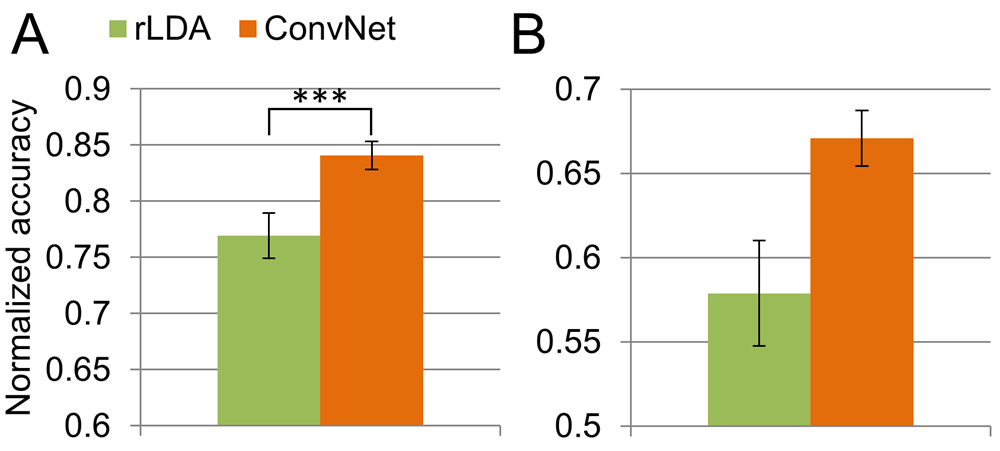
\includegraphics[width=.45\linewidth]{images/within-subject-flanker-gui.png}} \quad
    \subfloat[\textbf{Mean normalized decoding accuracy on unknown subjects.} Error bars show the SEM. A) Eriksen flanker task, trained on 30 subjects, tested on 1 subject.  Deep ConvNets were 5.05\% better than rLDA, p = 3.16 *10-4 (paired t-test). B) Online GUI control. Trained on 3 subjects, tested on the  respective remaining subject. Figure from {cite:t}`volker2018deep`.]
    {\label{cross-subject-flanker-gui-fig}
        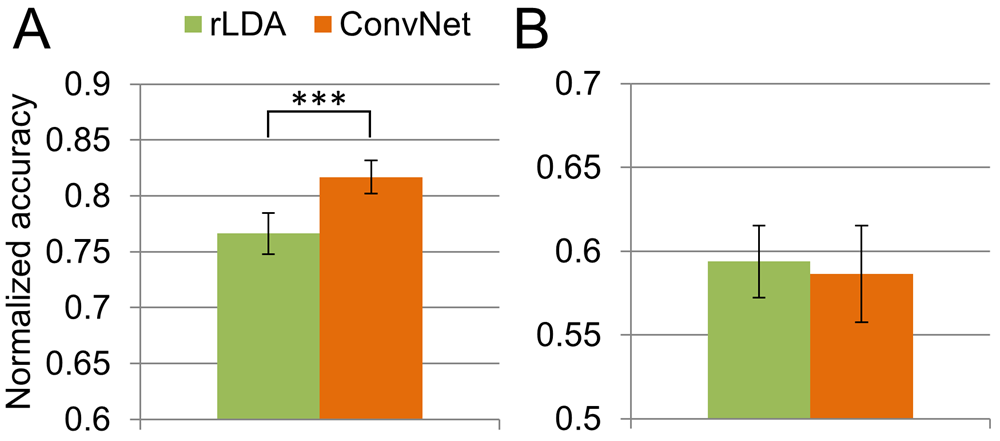
\includegraphics[width=.45\linewidth]{images/cross-subject-flanker-gui.png}} 
    \caption[Error decoding accuracy on Eriksen flanker task and online GUI control]{\textbf{Error decoding accuracy on Eriksen flanker task and online GUI control.}}
\end{figure}


    In two additional error-related decoding experiments, we evaluated an
Eriksen flanker task and errors during an the online control of a
graphical user interface through a brain-computer-interface. In the
Eriksen flanker task, the subjects were asked to press the left or right
button on a gamepad depending on whether an `L' or an `R' was the middle
character of a 5-letter string displayed on the screen. For the online
graphical user interface (GUI) control, the subjects were given an aim
to reach using the GUI, also see \Cref{online-bci}. They had to
think of one of the classes of the aforementioned Mixed Imagery Dataset
to choose one of four possible GUI actions. The correct GUI action was
always determined by the specificed aim given to the subject, hence an
erroneous action could be detected. The decoding task in this paper was
to distinguish whether the BCI-selected action was correct or erroneous.
Results in \Cref{within-subject-flanker-gui-fig} and
\Cref{cross-subject-flanker-gui-fig} show that deep ConvNets
outperform rLDA in all settings except cross-subject error-decoding for
online GUI control, where the low number of subjects (4) may prevent the
ConvNets to learn enough to outperform rLDA.

\section{Proof-of-Concept Assistive
System}\label{proof-of-concept-assistive-system}


\begin{figure}[htb]
    \myfloatalign
    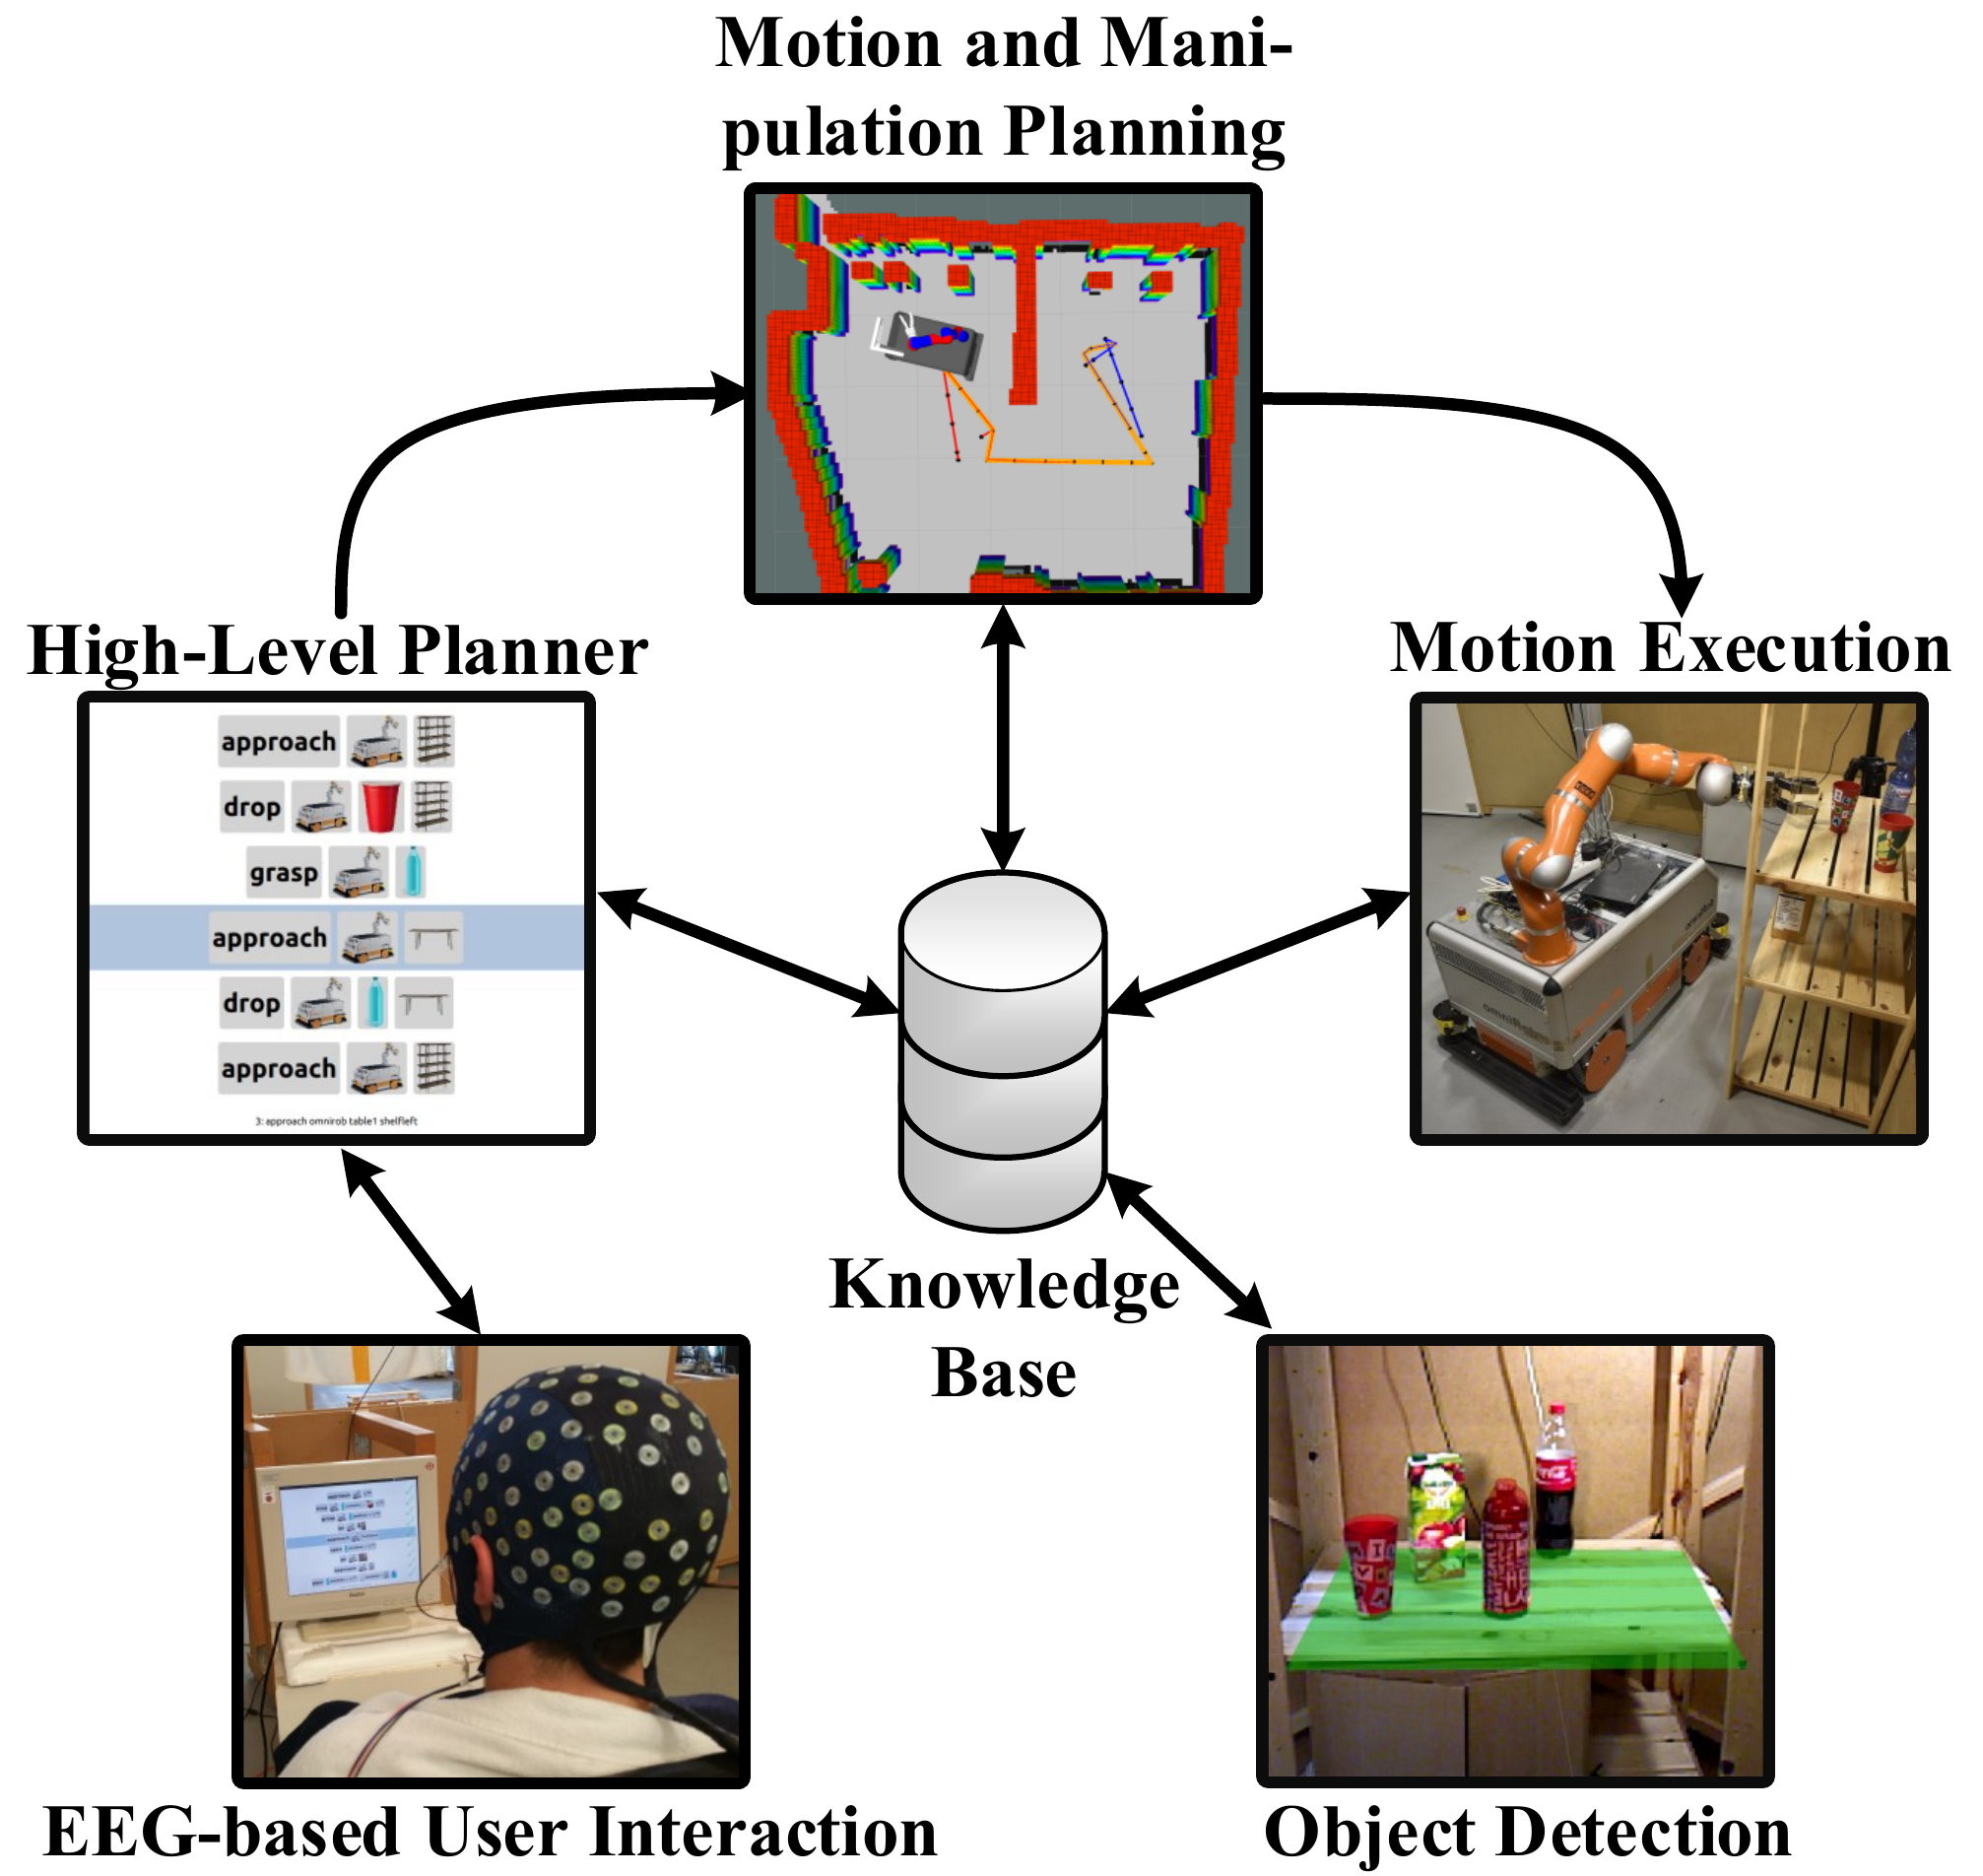
\includegraphics[width=0.7\linewidth]{images/robot-bci-overview.png}
    \caption[Overview of the proof-of-concept assistive system]{
\textbf{Overview of the proof-of-concept assistive system. The system
uses the deep ConvNet in the BCI component.} Robotic arm could be given high-level commands via the BCI, high-level commands were extracted from a knowledge base. The commands were then autonomously planned and executed by the robotic arm. Figure
from \citet{burget2017acting}
}
\label{robot-bci-overview-fig}
\end{figure}



\begin{table}[htb]
    \myfloatalign
    \footnotesize
    \begin{tabularx}{\textwidth}{p{0.1\textwidth}p{0.1\textwidth}p{0.1\textwidth}p{0.1\textwidth}p{0.1\textwidth}p{0.1\textwidth}p{0.1\textwidth}}
    \toprule
        \tableheadlinewithwidth{0.11\textwidth}{Subject} &
        \tableheadlinewithwidth{0.11\textwidth}{Runs} &
        \tableheadlinewithwidth{0.11\textwidth}{Accu-racy [\%] } &
        \tableheadlinewithwidth{0.11\textwidth}{Time {[}s{]}} &
        \tableheadlinewithwidth{0.11\textwidth}{Steps} &
        \tableheadlinewithwidth{0.11\textwidth}{Path Optimality {[}\%{]}} &
        \tableheadlinewithwidth{0.11\textwidth}{Time / Step {[}s{]}} \\ 
        \midrule
S1 & 18 & 84.1 ± 6.1 & 125 ± 84 & 13.0 ± 7.8 & 70.1 ± 22.3 & 9 ± 2 \\
S2 & 14 & 76.8 ± 14.1 & 150 ± 32 & 10.1 ± 2.8 & 91.3 ± 12.0 & 9 ± 3 \\
S3 & 17 & 82.0 ± 7.4 & 200 ± 159 & 17.6 ± 11.4 & 65.7 ± 28.9 & 11 ± 4 \\
S4 & 3 & 63.8 ± 15.6 & 176 ± 102 & 26.3 ± 11.2 & 34.5 ± 1.2 & 6 ± 2 \\
Average & 13 & 76.7 ± 9.1 & 148 ± 50 & 16.7 ± 7.1 & 65.4 ± 23.4 & 9 ±
2 \\
        \bottomrule
    \end{tabularx}
    \caption[Decoding problems in deep-learning EEG decoding studies prior to our work.]{
    \textbf{Results for BCI control of the GUI.} Accuracy is
fraction of correct commands, time is time per command, steps is steps
needed to reach the aim, path optimality is ratio of miniminally needed
nubmer of steps to actually used number of steps when every step is
optimal, and time/step is time per step. Results from 
\citet{burget2017acting}.
    }  \label{bci-robot-results}
\end{table}



    We also evaluated the use of our deep ConvNet as part of an assistive
robot system where the brain-computer interface was sending high-level
commands to a robotic arm. In this proof-of-concept system, the robotic
arm could be instructed by the user via the BCI to fetch a cup and
directly move the cup to the persons mouth to drink from it. An overview
can be seen in \Cref{robot-bci-overview-fig}. Results from
\Cref{bci-robot-results} show that 3 out of 4 subjects had a
command accuracy of more than 75\% and were able to reach the target
using less than twice the steps of the minimal path through the GUI
(path optimality \textgreater{} 50\%).

\section{Intracranial EEG Decoding}\label{intracranial-eeg-decoding}

\subsection{Intracranial EEG Decoding of Eriksen Flanker
Task}\label{intracranial-eeg-decoding-of-eriksen-flanker-task}


\begin{table}[htb]
    \myfloatalign
    \footnotesize
    \begin{tabularx}{\textwidth}{p{0.2\textwidth}p{0.2\textwidth}p{0.2\textwidth}p{0.2\textwidth}}
    \toprule
        \tableheadlinewithwidth{0.2\textwidth}{Classifier} &
        \tableheadlinewithwidth{0.2\textwidth}{Balanced Accuracy} &
        \tableheadlinewithwidth{0.2\textwidth}{Accuracy Correct Class } &
        \tableheadlinewithwidth{0.2\textwidth}{Accuracy Error Class} \\ 
        \midrule
Deep4Net & 59.28 ± 0.50 & 69.37 ± 0.44 & 49.19 ± 0.56 \\
ShallowNet & 58.42 ± 0.32 & 74.83 ± 0.25 & 42.01 ± 0.40 \\
EEGNet & 57.73 ± 0.52 & 57.78 ± 0.48 & 57.68 ± 0.56 \\
rLDA & 53.76 ± 0.32 & 76.12 ± 0.26 & 31.40 ± 0.38 \\
ResNet & 52.45 ± 0.21 & 95.47 ± 0.14 & 09.43 ± 0.28 \\
        \bottomrule
    \end{tabularx}
    \caption[Decoding problems in deep-learning EEG decoding studies prior to our work.]{
    \textbf{Results for single-channel intracranial decoding of
errors during an Eriksen flanker task.} Balanced Accuracy is the mean of
the accuracies for correct class ground truth labels and error class
ground truth labels. Results from 
\citet{intracranial-error-results-table}.
    }  \label{bci-robot-results}
\end{table}
 

\begin{figure}[htb]
    \myfloatalign
    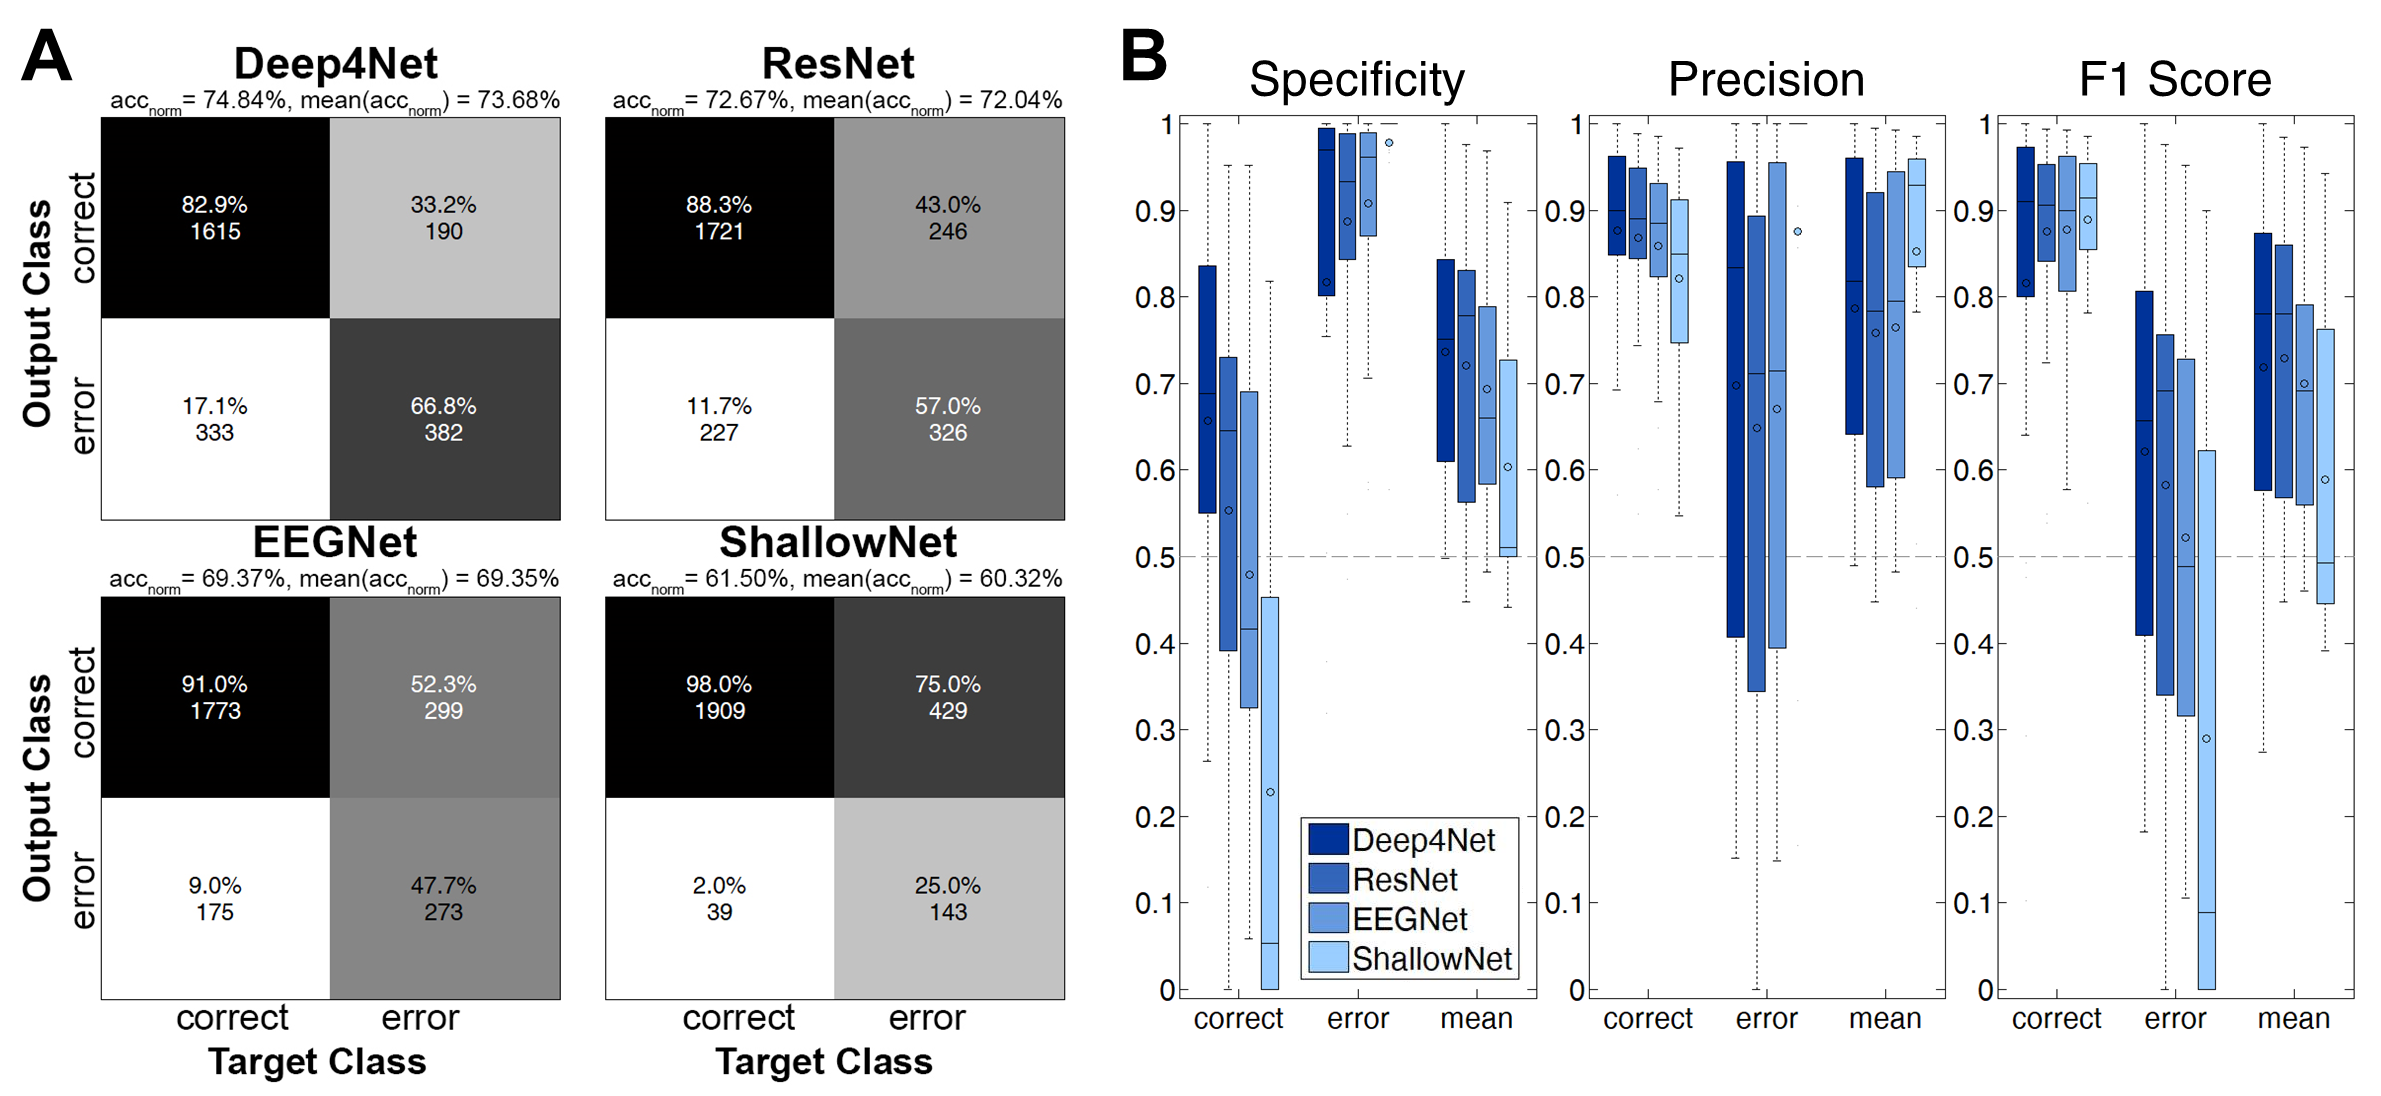
\includegraphics[width=1\linewidth]{images/IntracranialError.png}
    \caption[Results for all-channel intracranial decoding of errors during
an Eriksen flanker task]{
\textbf{Results for all-channel intracranial decoding of errors during
an Eriksen flanker task.} Here, the classifiers were trained on all
available channels per patient. A) Confusion matrices of the four models
used for decoding. The matrices display the sum of all trials over the
24 recordings. On top of the matrices, the class-normalized accuracy
(average over per-class accuracies) over all trials, i.e.,
$\mathrm{acc}_\mathrm{norm}$, and the mean of the single recordings'
normalized accuracy, i.e., $\mathrm{mean}(\mathrm{acc}_\mathrm{norm})$
is displayed; please note that these two measures differ slightly, as
the patients had a varying number of total trials and trials per class.
B) Box plots for specificity, precision and F1 score. The box represents
the interquartile range (IQR) of the data, the circle within the mean,
the horizontal line depicts the median. The lower whiskers include all
data points that have the minimal value of
$25^\mathrm{th} \mathrm{percentile}-1.5 \cdot \mathrm{IQR}$, the upper
whiskers include all points that are maximally
$75^\mathrm{th} \mathrm{percentile}+1.5 \cdot \mathrm{IQR}$. Figure
from \citet{volker2018intracranial}.
}
\label{intracranial-error-results-fig}
\end{figure}

    We further evaluated whether the same networks developed for noninvasive
EEG decoding can successfully learn to decode intracranial EEG.
Therefore, in one work we used the same Eriksen flanker task as
described in \Cref{flanker-and-gui-section}, but recorded
intracranial EEG from 23 patients who had pharmacoresistant epilepsy
\cite{volker2018intracranial}. Results for single-channel
decoding \Cref{intracranial-error-results-table} show the
deep and shallow ConvNet to clearly outperform rLDA (59.3\%/58.4\%
vs.~53.8\%) , whereas the residual ConvNet has low accuracy (52.5\%). In
contrast, results for all-channel decoding
\Cref{intracranial-error-results-fig} show the residual
ConvNet to perform well with the residual ConvNet and the deep ConvNet
outperforming the shallow ConvNet (72.1\% and 73.7\% vs.~60.3\%
class-normalized accuracies (average over per-class accuracies)).

\subsection{Transfer Learning for Intracranial Error
Decoding}\label{transfer-learning-for-intracranial-error-decoding}

\begin{figure}[htb]
    \myfloatalign
    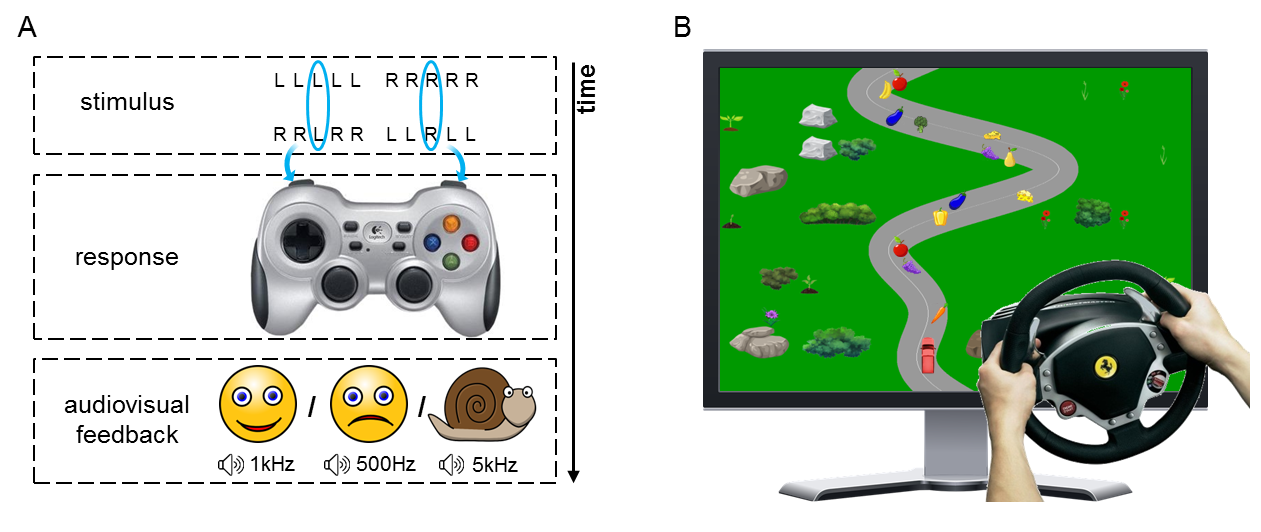
\includegraphics[width=1\linewidth]{images/eriksen-flanker-car-driving-tasks.png}
    \caption[Visualizations of Eriksen flanker and  car driving task]{
\textbf{Sketch of the Eriksen flanker task (A) and screenshot of the car
driving task (B).} Figure from \citet{behncke2018cross}. 
}
\label{eriksen-flanker-car-driving-tasks-fig}
\end{figure}


\begin{figure}[htb]
    \myfloatalign
    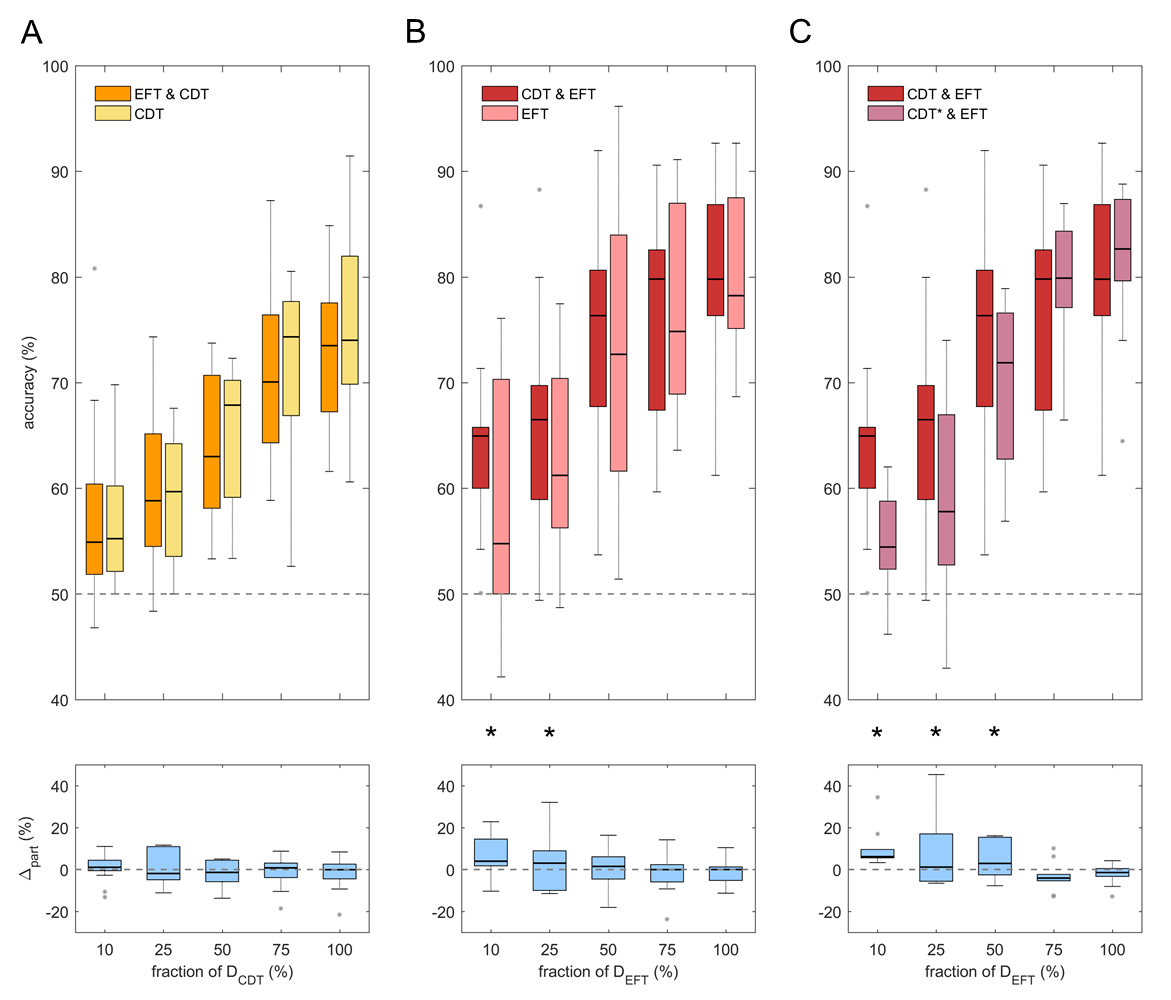
\includegraphics[width=1\linewidth]{images/cross-training-eft-cdt-results.png}
    \caption[Results for transfer learning on the Eriksen flanker task and the car driving task]{

\textbf{Results for transfer learning on the Eriksen flanker task (EFT)
and the car driving task (CDT).} All results are computed for a varying
fraction of available data for the target decoding task (bottom row).
\textbf{A} compares CDT accuracies after training only on CDT or
pretraining on EFT and finetuning on CDT. \textbf{B} compares EFT
accuracies after only training on EFT or after pretraining on CDT and
finetuning on EFT. As a sanity check for the results in \textbf{B},
\textbf{C} compares EFT accuracies when pretraining on original CDT data
and finetuning on EFT to pretraining on CDT data with shuffled labels
(CDT*) and finetuning on EFT. Results show that pretraining on CDT helps
EFT decoding when little EFT data is available. Figure from
\citet{behncke2018cross}.
}
\label{cross-training-eft-cdt-results-fig}
\end{figure}


    We further tested the potential of ConvNets to transfer knowledge
learned from decoding intracranial signals in error-decoding paradigm to
decoding signals in another a different error-decoding paradigm
\cite{behncke2018cross}. The two error-decoding paradigms were
the aforementioned Eriksen flanker task (EFT) and a car driving task
(CDT), where subjects had to use a steering wheel to steer a car in a
computer game and avoid hitting obstacles, where hitting an obstacle was
considered an error event (see
\Cref{eriksen-flanker-car-driving-tasks-fig}). Results in
\Cref{cross-training-eft-cdt-results-fig} show that
pretraining on CDT helps EFT decoding when few EDT data is available.

\subsection{Microelectrocorticography Decoding of Auditory Evoked
Responses in
Sheep}\label{microelectrocorticography-decoding-of-auditory-evoked-responses-in-sheep}

\begin{figure}[htb]
    \myfloatalign
    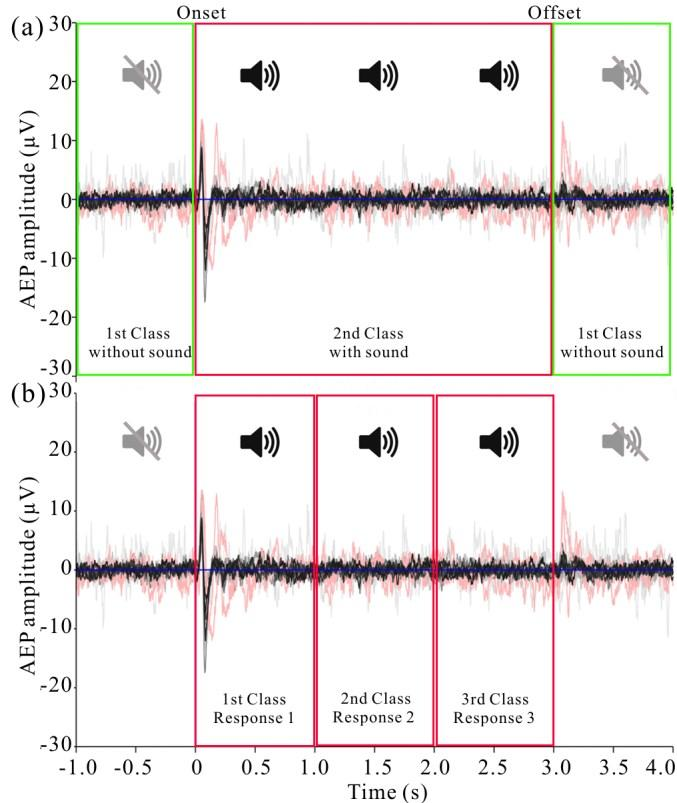
\includegraphics[width=0.65\linewidth]{images/sheep-sounds.jpg}
    \caption[Overview over decoding tasks for
auditory evoked responses in a sheep]{
\textbf{Overview over decoding tasks for
auditory evoked responses in a sheep.} First task (top) was to
distingish 3 seconds when the sound was playing from the second before
and the second after. Second task (bottom) was to distinguish the first,
second and third second during theplaying of the sound. Signals are
averaged responses from one electrode during different days, with black
and grey being signals while the sheep was awake and red ones while the
sheep was under general anesthesia. Figure from \citet{wangsheep}.
}
\label{sheep-sounds-fig}
\end{figure}


\begin{figure}[htb]
    \myfloatalign
    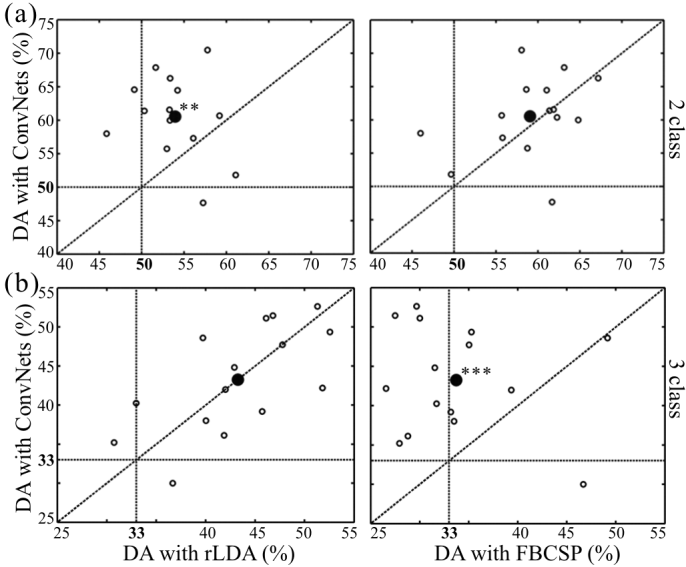
\includegraphics[width=0.65\linewidth]{images/sheep-accuracies.png}
    \caption[Results of decoding auditory evoked responses]{
\textbf{Results of decoding auditory evoked responses from sheep.}
rlDA, FBSCP and the deep ConvNet were the decoding models. Open circles represent accuracies for individual experiment days and closed circles represent the average
over these accuracies. Figure from \citet{wangsheep}.
}
\label{sheep-accuracies-fig}
\end{figure}



    In this study, we evaluated the ConvNets for decoding auditory evoked
responses played to a sheep that was chronically implanted with a 

$\mu$ECoG-based neural interfacing device \cite{wangsheep}.

3-seconds-long sounds were presented to the sheep and two decoding tasks
were defined from those 3 seconds as well as the second immediately
before and after the playing of the sound. The first decoding task was
to distinguish the 3 seconds when the sound was playing from the second
immediately before and the second immediately after the sound. The
second task was distinguishing the first, second and third second of the
playing of the sound to discriminate early, intermediate and late
auditory evoked response (see \Cref{sheep-sounds-fig}).
Results in \Cref{sheep-accuracies-fig} show that the deep
ConvNet can perform as good as FBSCP and rLDA, and perform well on both
tasks, whereas rLDA performs competitively only on the first and FBSCP
only on the second task.

\section{Evaluation on Large-Scale Task-Diverse
Dataset}\label{evaluation-on-large-scale-task-diverse-dataset}


\begin{table}[htb]
    \myfloatalign
    \footnotesize
    \begin{tabularx}{\textwidth}{p{0.2\textwidth}p{0.1\textwidth}p{0.2\textwidth}p{0.1\textwidth}p{0.1\textwidth}p{0.1\textwidth}}
    \toprule
        \tableheadlinewithwidth{0.2\textwidth}{Name (Acronym)} &
        \tableheadlinewithwidth{0.1\textwidth}{\#Classes} &
        \tableheadlinewithwidth{0.2\textwidth}{Task type} &
        \tableheadlinewithwidth{0.1\textwidth}{\#Sub-jects}&
        \tableheadlinewithwidth{0.1\textwidth}{Trials per subject}&
        \tableheadlinewithwidth{0.1\textwidth}{Class balance} \\ 
        \midrule
High-Gamma Dataset (Motor) & 4 & Motor task & 20 & 1000 & balanced \\
KUKA Pouring Observation (KPO) & 2 & Error observation & 5 & 720-800 &
balanced \\
Robot-Grasping Observation (RGO) & 2 & Error observation & 12 & 720-800
& balanced \\
Error-Related Negativity (ERN) & 2 & Eriksen flanker task & 31 & 1000 &
1/2 up to 1/15 \\
Semantic Categories & 3 & Speech imagery & 16 & 750 & balanced \\
Real vs.~Pseudo Words & 2 & Speech imagery & 16 & 1000 & 3/1 \\
        \bottomrule
    \end{tabularx}
    \caption[Datasets for the large-scale evaluation framework]{
    \textbf{Datasets for the large-scale evaluation framework.} Used in \citet{heilmeyer2018large}.
    }  \label{large-framework-overview-table}
\end{table}


\begin{figure}[htb]
    \myfloatalign
    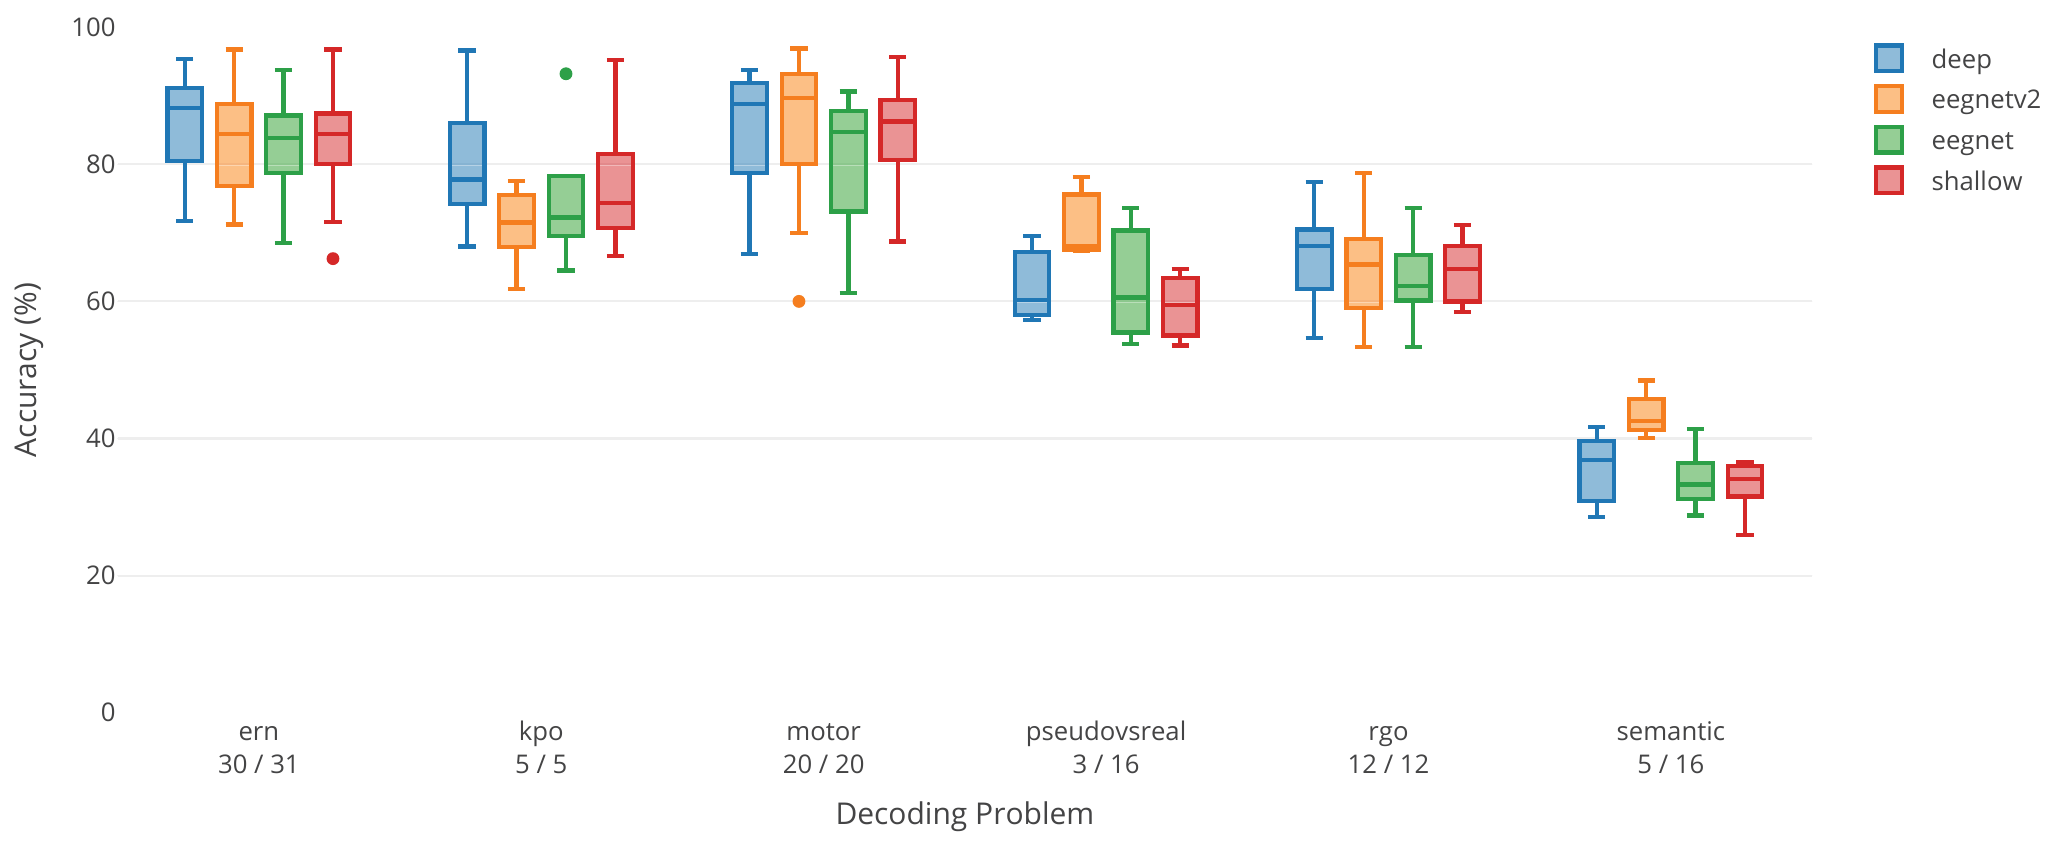
\includegraphics[width=1\linewidth]{images/large-framework-per-dataset-results.png}
    \caption[Large-scale evaluation results]{
\textbf{Per-dataset results for the large-scale evaluation of deep
ConvNet, shallow ConvNet and two versions of EEGNet.} Boxplots show the
distribution over per-subject accuracies for the individual decoding
tasks. ern, kpo and rgo are the error-related datasets, ern:
Error-related negativity Eriksen flanker task, KPO: KUKA Pouring
Observation paradigm, rgo: robot-grasping observation paradigm. motor is
the high-gamma dataset with 6 additional subjects that were excluded for
data quality reasons from \cite{schirrmeisterdeephbm2017}.
pseudovsreal and semantic are two semantic processing datasets to
classify silent repetitions of pseudowords vs.~realwords (pseudovsreal)
or different semantic categories (semantic) . Figure from
\citet{heilmeyer2018large}.
}
\label{large-framework-per-dataset-results-fig}
\end{figure}


\begin{figure}[htb]
    \myfloatalign
    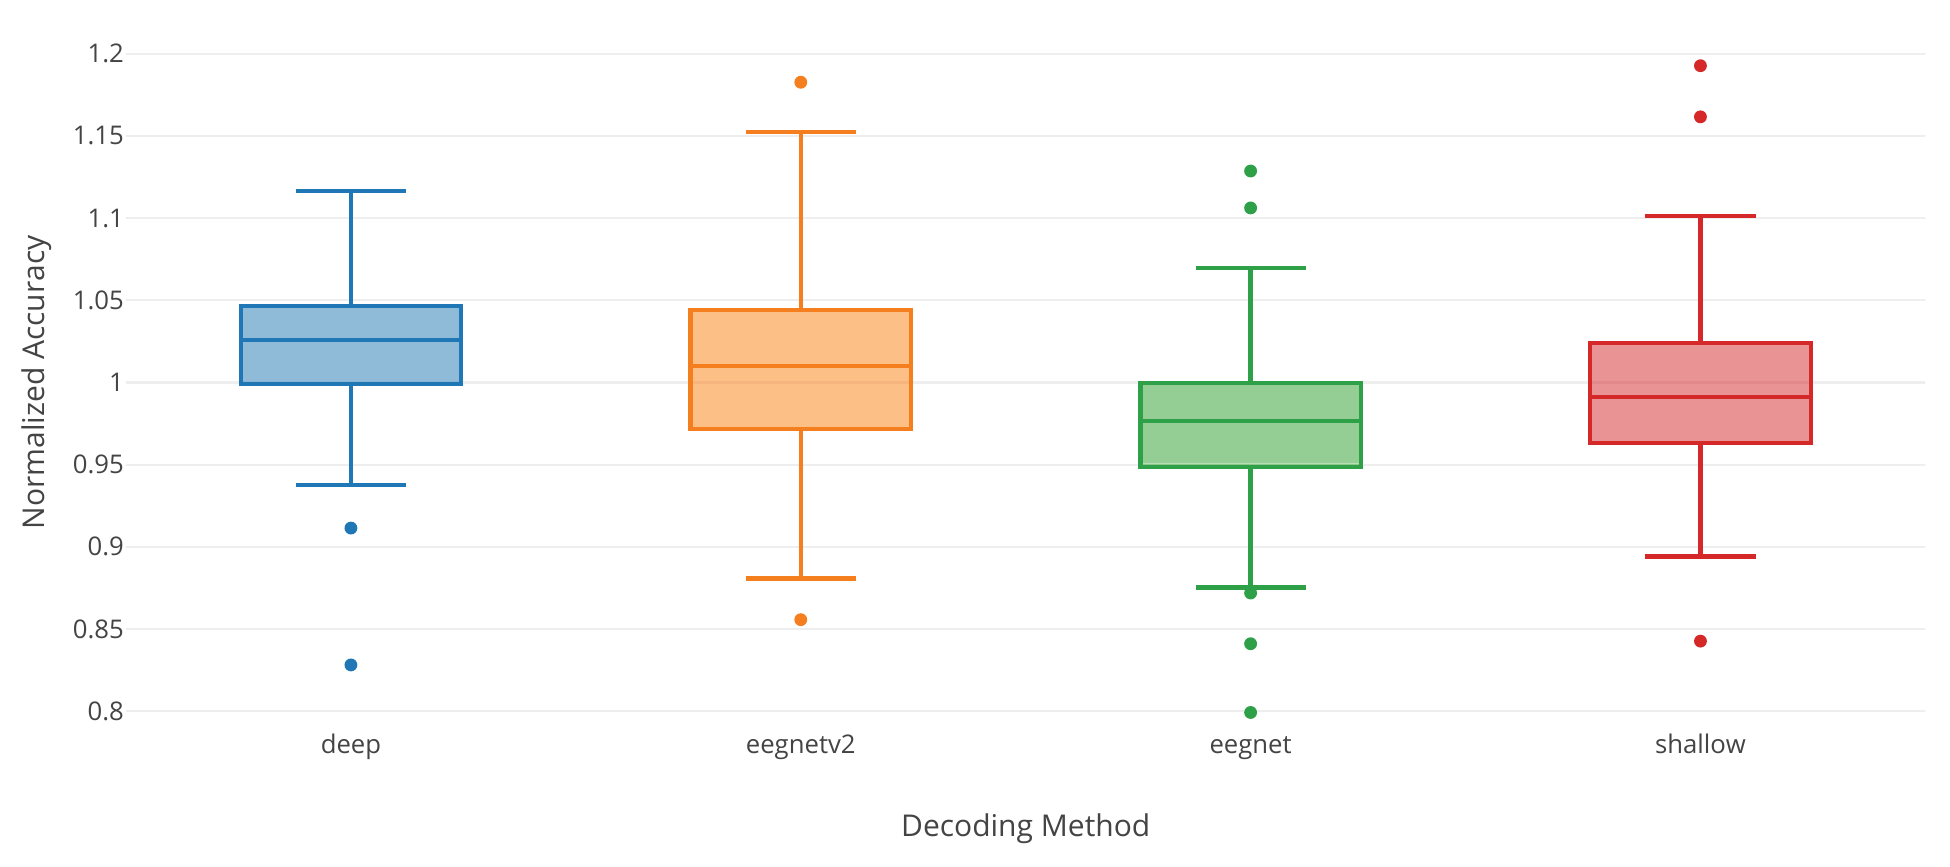
\includegraphics[width=1\linewidth]{images/large-framework-averaged-results.png}
    \caption[Large-scale dataset-averaged evaluation results]{
\textbf{Dataset-averaged results for the large-scale evaluation of deep
ConvNet, shallow ConvNet and two versions of EEGNet.} Accuracies are
normalized to the average of the accuracies of all models. Figure from
\citet{heilmeyer2018large}.
}
\label{large-framework-averaged-results-fig}
\end{figure}


\begin{table}[htb]
    \myfloatalign
    \footnotesize
    \begin{tabularx}{\textwidth}{p{0.3\textwidth}p{0.3\textwidth}p{0.3\textwidth}}
    \toprule
        \tableheadlinewithwidth{0.3\textwidth}{Network} &
        \tableheadlinewithwidth{0.3\textwidth}{Mean accuracy} &
        \tableheadlinewithwidth{0.3\textwidth}{Mean normalized accuracy} \\ 
        \midrule
Deep ConvNet & 70.08\% ± 20.92\% & 1.00 ± 0.05 \\
EEGNetv2 & 70.00\% ±18.86\% & 1.02 ± 0.08 \\
EEGNet & 67.71\% ± 19.04\% & 0.98 ± 0.06 \\
Shallow ConvNet & 67.71\% ±19.04\% & 0.99 ± 0.06 \\
        \bottomrule
    \end{tabularx}
    \caption[Datasets for the large-scale evaluation framework]{
    \textbf{Dataset-averaged results for the large-scale
evaluation of deep ConvNet, shallow ConvNet and two versions of EEGNet.}
Accuracies are normalized to the average of the accuracies of all
models. Results from \citet{heilmeyer2018large}.
    }  \label{large-framework-results-table}
\end{table}




We also compared the deep and shallow ConvNet architectures as well as
EEGNet on six classification tasks with more than 90000 trials in total
(see \Cref{large-framework-overview-table})
\citep{heilmeyer2018large}. The datasets tasks were all
recorded in our lab and included the high-gamma dataset, three
error-related tasks described before (Eriksen flanker task, robot
grasping and robot pouring observations) as well as two tasks on
semantic processing. In the semantic processing dataset, the
classification tasks were to distinguish different types of words that a
subject silently repeated \cite{Rau:2015uk}. The first task
was to distinguish existing real words from nonexisting pseudowords. The
second classification task was to distingiush three semantic categories
(food, animals, tools) the word may belong to. The evaluation code for
all models always used the original code and hyperparameters from the
original studies in order to ensure a fair comparison. Results show that
the deep ConvNet and the more recent version of EEGNet (EEGNetv2)
perform similarly well, with shallow and an older version of EEGNet
performing slightly worse, see
\Cref{large-framework-per-dataset-results-fig},
\Cref{large-framework-averaged-results-fig} and
\Cref{large-framework-results-table}.

\begin{openbox}
\item How do these networks perform on non-trial-based tasks like pathology decoding?
\end{openbox}
